% Options for packages loaded elsewhere
\PassOptionsToPackage{unicode}{hyperref}
\PassOptionsToPackage{hyphens}{url}
%
\documentclass[
]{article}
\usepackage{amsmath,amssymb}
\usepackage{lmodern}
\usepackage{iftex}
\ifPDFTeX
  \usepackage[T1]{fontenc}
  \usepackage[utf8]{inputenc}
  \usepackage{textcomp} % provide euro and other symbols
\else % if luatex or xetex
  \usepackage{unicode-math}
  \defaultfontfeatures{Scale=MatchLowercase}
  \defaultfontfeatures[\rmfamily]{Ligatures=TeX,Scale=1}
\fi
% Use upquote if available, for straight quotes in verbatim environments
\IfFileExists{upquote.sty}{\usepackage{upquote}}{}
\IfFileExists{microtype.sty}{% use microtype if available
  \usepackage[]{microtype}
  \UseMicrotypeSet[protrusion]{basicmath} % disable protrusion for tt fonts
}{}
\makeatletter
\@ifundefined{KOMAClassName}{% if non-KOMA class
  \IfFileExists{parskip.sty}{%
    \usepackage{parskip}
  }{% else
    \setlength{\parindent}{0pt}
    \setlength{\parskip}{6pt plus 2pt minus 1pt}}
}{% if KOMA class
  \KOMAoptions{parskip=half}}
\makeatother
\usepackage{xcolor}
\usepackage[margin=1in]{geometry}
\usepackage{color}
\usepackage{fancyvrb}
\newcommand{\VerbBar}{|}
\newcommand{\VERB}{\Verb[commandchars=\\\{\}]}
\DefineVerbatimEnvironment{Highlighting}{Verbatim}{commandchars=\\\{\}}
% Add ',fontsize=\small' for more characters per line
\usepackage{framed}
\definecolor{shadecolor}{RGB}{248,248,248}
\newenvironment{Shaded}{\begin{snugshade}}{\end{snugshade}}
\newcommand{\AlertTok}[1]{\textcolor[rgb]{0.94,0.16,0.16}{#1}}
\newcommand{\AnnotationTok}[1]{\textcolor[rgb]{0.56,0.35,0.01}{\textbf{\textit{#1}}}}
\newcommand{\AttributeTok}[1]{\textcolor[rgb]{0.77,0.63,0.00}{#1}}
\newcommand{\BaseNTok}[1]{\textcolor[rgb]{0.00,0.00,0.81}{#1}}
\newcommand{\BuiltInTok}[1]{#1}
\newcommand{\CharTok}[1]{\textcolor[rgb]{0.31,0.60,0.02}{#1}}
\newcommand{\CommentTok}[1]{\textcolor[rgb]{0.56,0.35,0.01}{\textit{#1}}}
\newcommand{\CommentVarTok}[1]{\textcolor[rgb]{0.56,0.35,0.01}{\textbf{\textit{#1}}}}
\newcommand{\ConstantTok}[1]{\textcolor[rgb]{0.00,0.00,0.00}{#1}}
\newcommand{\ControlFlowTok}[1]{\textcolor[rgb]{0.13,0.29,0.53}{\textbf{#1}}}
\newcommand{\DataTypeTok}[1]{\textcolor[rgb]{0.13,0.29,0.53}{#1}}
\newcommand{\DecValTok}[1]{\textcolor[rgb]{0.00,0.00,0.81}{#1}}
\newcommand{\DocumentationTok}[1]{\textcolor[rgb]{0.56,0.35,0.01}{\textbf{\textit{#1}}}}
\newcommand{\ErrorTok}[1]{\textcolor[rgb]{0.64,0.00,0.00}{\textbf{#1}}}
\newcommand{\ExtensionTok}[1]{#1}
\newcommand{\FloatTok}[1]{\textcolor[rgb]{0.00,0.00,0.81}{#1}}
\newcommand{\FunctionTok}[1]{\textcolor[rgb]{0.00,0.00,0.00}{#1}}
\newcommand{\ImportTok}[1]{#1}
\newcommand{\InformationTok}[1]{\textcolor[rgb]{0.56,0.35,0.01}{\textbf{\textit{#1}}}}
\newcommand{\KeywordTok}[1]{\textcolor[rgb]{0.13,0.29,0.53}{\textbf{#1}}}
\newcommand{\NormalTok}[1]{#1}
\newcommand{\OperatorTok}[1]{\textcolor[rgb]{0.81,0.36,0.00}{\textbf{#1}}}
\newcommand{\OtherTok}[1]{\textcolor[rgb]{0.56,0.35,0.01}{#1}}
\newcommand{\PreprocessorTok}[1]{\textcolor[rgb]{0.56,0.35,0.01}{\textit{#1}}}
\newcommand{\RegionMarkerTok}[1]{#1}
\newcommand{\SpecialCharTok}[1]{\textcolor[rgb]{0.00,0.00,0.00}{#1}}
\newcommand{\SpecialStringTok}[1]{\textcolor[rgb]{0.31,0.60,0.02}{#1}}
\newcommand{\StringTok}[1]{\textcolor[rgb]{0.31,0.60,0.02}{#1}}
\newcommand{\VariableTok}[1]{\textcolor[rgb]{0.00,0.00,0.00}{#1}}
\newcommand{\VerbatimStringTok}[1]{\textcolor[rgb]{0.31,0.60,0.02}{#1}}
\newcommand{\WarningTok}[1]{\textcolor[rgb]{0.56,0.35,0.01}{\textbf{\textit{#1}}}}
\usepackage{graphicx}
\makeatletter
\def\maxwidth{\ifdim\Gin@nat@width>\linewidth\linewidth\else\Gin@nat@width\fi}
\def\maxheight{\ifdim\Gin@nat@height>\textheight\textheight\else\Gin@nat@height\fi}
\makeatother
% Scale images if necessary, so that they will not overflow the page
% margins by default, and it is still possible to overwrite the defaults
% using explicit options in \includegraphics[width, height, ...]{}
\setkeys{Gin}{width=\maxwidth,height=\maxheight,keepaspectratio}
% Set default figure placement to htbp
\makeatletter
\def\fps@figure{htbp}
\makeatother
\setlength{\emergencystretch}{3em} % prevent overfull lines
\providecommand{\tightlist}{%
  \setlength{\itemsep}{0pt}\setlength{\parskip}{0pt}}
\setcounter{secnumdepth}{-\maxdimen} % remove section numbering
\ifLuaTeX
  \usepackage{selnolig}  % disable illegal ligatures
\fi
\IfFileExists{bookmark.sty}{\usepackage{bookmark}}{\usepackage{hyperref}}
\IfFileExists{xurl.sty}{\usepackage{xurl}}{} % add URL line breaks if available
\urlstyle{same} % disable monospaced font for URLs
\hypersetup{
  pdftitle={HUDM6026 Homework\_05},
  pdfauthor={Chenguang Pan \& Seng Lei},
  hidelinks,
  pdfcreator={LaTeX via pandoc}}

\title{HUDM6026 Homework\_05}
\author{Chenguang Pan \& Seng Lei}
\date{Feb 24, 2023}

\begin{document}
\maketitle

\hypertarget{q1}{%
\subsection{Q1:}\label{q1}}

\emph{Determine the first derivative of f and encode it in a function
called f\_prime.}

\textbf{MY SOLUTION:}\\
Based on chain rule, the first derivative of \(f(x)\) is
\[f(x)' = \frac{-2x}{x^2+1}+\frac{1}{3}x^{-\frac{2}{3}}\]. Based on this
equation, I write the code below. Certainly, we can use the R-built-in
function to get the derivative quickly.

\begin{Shaded}
\begin{Highlighting}[]
\SpecialCharTok{\textgreater{}}\NormalTok{ f\_prime }\OtherTok{\textless{}{-}} \ControlFlowTok{function}\NormalTok{(x) \{}
\SpecialCharTok{+}\NormalTok{   out\_ }\OtherTok{\textless{}{-}}\NormalTok{ (}\SpecialCharTok{{-}}\DecValTok{2}\SpecialCharTok{*}\NormalTok{x)}\SpecialCharTok{*}\NormalTok{((x}\SpecialCharTok{\^{}}\DecValTok{2} \SpecialCharTok{+} \DecValTok{1}\NormalTok{)}\SpecialCharTok{\^{}}\NormalTok{(}\SpecialCharTok{{-}}\DecValTok{1}\NormalTok{)) }\SpecialCharTok{+}\NormalTok{ (}\DecValTok{1}\SpecialCharTok{/}\DecValTok{3}\NormalTok{)}\SpecialCharTok{*}\NormalTok{(x}\SpecialCharTok{\^{}}\NormalTok{(}\SpecialCharTok{{-}}\DecValTok{2}\SpecialCharTok{/}\DecValTok{3}\NormalTok{))}
\SpecialCharTok{+}   \FunctionTok{return}\NormalTok{(out\_)}
\SpecialCharTok{+}\NormalTok{ \}}
\end{Highlighting}
\end{Shaded}

\hypertarget{q2}{%
\subsection{Q2:}\label{q2}}

\emph{Create a plot of f and f on {[}0,4{]} in different colors and line
types and add a legend.} \textbf{MY SOLUTION:}

\begin{Shaded}
\begin{Highlighting}[]
\SpecialCharTok{\textgreater{}} \CommentTok{\# write the original function with the name of f\_}
\ErrorTok{\textgreater{}}\NormalTok{ f\_ }\OtherTok{\textless{}{-}} \ControlFlowTok{function}\NormalTok{(x)\{}
\SpecialCharTok{+}\NormalTok{   out\_ }\OtherTok{\textless{}{-}}\NormalTok{ (}\SpecialCharTok{{-}}\DecValTok{1}\NormalTok{)}\SpecialCharTok{*}\FunctionTok{log}\NormalTok{(x}\SpecialCharTok{\^{}}\DecValTok{2} \SpecialCharTok{+} \DecValTok{1}\NormalTok{) }\SpecialCharTok{+}\NormalTok{ x}\SpecialCharTok{\^{}}\NormalTok{(}\DecValTok{1}\SpecialCharTok{/}\DecValTok{3}\NormalTok{)}
\SpecialCharTok{+}   \FunctionTok{return}\NormalTok{(out\_)\}}
\SpecialCharTok{\textgreater{}} \FunctionTok{f\_}\NormalTok{(}\DecValTok{1}\NormalTok{)}
\NormalTok{[}\DecValTok{1}\NormalTok{] }\FloatTok{0.3068528}
\SpecialCharTok{\textgreater{}} \CommentTok{\# first plot the original function}
\ErrorTok{\textgreater{}}\NormalTok{ x }\OtherTok{\textless{}{-}} \FunctionTok{seq}\NormalTok{(}\DecValTok{0}\NormalTok{,}\DecValTok{4}\NormalTok{,}\FloatTok{0.01}\NormalTok{)}
\SpecialCharTok{\textgreater{}} \CommentTok{\# plot the original function with blue line}
\ErrorTok{\textgreater{}} \FunctionTok{plot}\NormalTok{(x, }\FunctionTok{f\_}\NormalTok{(x), }\AttributeTok{col=}\StringTok{"blue"}\NormalTok{, }\AttributeTok{type =} \StringTok{"l"}\NormalTok{, }\AttributeTok{ylim =} \FunctionTok{c}\NormalTok{(}\SpecialCharTok{{-}}\FloatTok{1.5}\NormalTok{,}\DecValTok{1}\NormalTok{))}
\SpecialCharTok{\textgreater{}} \CommentTok{\# plot the first derivative with red line}
\ErrorTok{\textgreater{}} \FunctionTok{lines}\NormalTok{(x, }\FunctionTok{f\_prime}\NormalTok{(x), }\AttributeTok{col=}\StringTok{"red"}\NormalTok{, }\AttributeTok{type =} \StringTok{"l"}\NormalTok{)}
\SpecialCharTok{\textgreater{}} \CommentTok{\# add the legend}
\ErrorTok{\textgreater{}} \FunctionTok{legend}\NormalTok{(}\DecValTok{3}\NormalTok{,}\DecValTok{1}\NormalTok{, }\AttributeTok{inset =} \FloatTok{0.1}\NormalTok{, }\FunctionTok{c}\NormalTok{(}\StringTok{"f\_"}\NormalTok{,}\StringTok{"f\_prime"}\NormalTok{), }\AttributeTok{lty =} \DecValTok{1}\NormalTok{, }
\SpecialCharTok{+}        \AttributeTok{col =} \FunctionTok{c}\NormalTok{(}\StringTok{"blue"}\NormalTok{,}\StringTok{"red"}\NormalTok{), }\AttributeTok{title=}\StringTok{"line Type"}\NormalTok{)}
\SpecialCharTok{\textgreater{}} \CommentTok{\# add a horizontal line to indicate the y=0}
\ErrorTok{\textgreater{}} \FunctionTok{abline}\NormalTok{(}\AttributeTok{h=}\DecValTok{0}\NormalTok{,}\AttributeTok{lty=}\DecValTok{3}\NormalTok{)}
\end{Highlighting}
\end{Shaded}

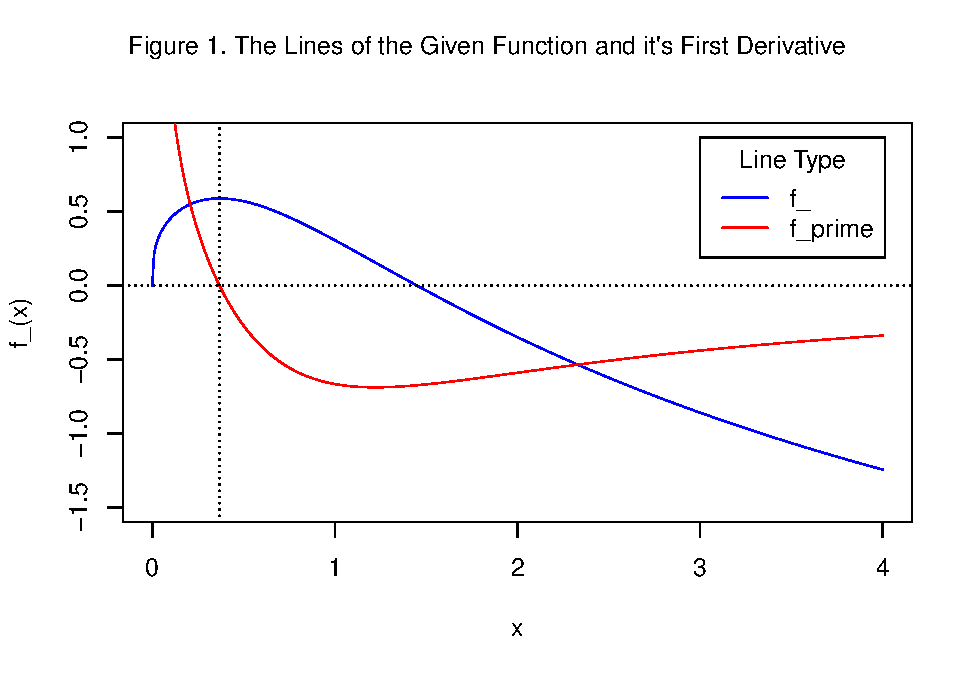
\includegraphics{Homework_05_Pan-Lei_files/figure-latex/unnamed-chunk-2-1.pdf}

\hypertarget{q3}{%
\subsection{Q3:}\label{q3}}

\emph{Finish the functions that I started in the R code notes for
univariate optimization for the golden section search, the bisection
method, and Newton's method.}

\textbf{MY SOLUTION:}\\
\#\#\# 3.1 The Golden Section Search

\begin{Shaded}
\begin{Highlighting}[]
\SpecialCharTok{\textgreater{}} \DocumentationTok{\#\#\#\#\#\#\#\#\#\#\#\#\#\#\#\#\#\#\#\#\#\#\#\#\#\#\#\#\#\#\#\#\#\#\#\#\#\#\#\#\#\#\#\#\#\#\#\#\#\#\#\#\#\#\#\#\#\#}
\ErrorTok{\textgreater{}} \DocumentationTok{\#\#\#\#\#\#\# FUNCTION TO DO THE GOLDEN SECTION SEARCH \#\#\#\#\#\#\#\#\#}
\ErrorTok{\textgreater{}} \DocumentationTok{\#\#\#\#\#\#\#\#\#\#\#\#\#\#\#\#\#\#\#\#\#\#\#\#\#\#\#\#\#\#\#\#\#\#\#\#\#\#\#\#\#\#\#\#\#\#\#\#\#\#\#\#\#\#\#\#\#\#}
\ErrorTok{\textgreater{}}\NormalTok{ golden }\OtherTok{\textless{}{-}} \ControlFlowTok{function}\NormalTok{(f, int, }\AttributeTok{precision =} \FloatTok{1e{-}6}\NormalTok{)}
\SpecialCharTok{+}\NormalTok{ \{}
\SpecialCharTok{+}   \CommentTok{\# ::: This function implements the golden section search for a }
\SpecialCharTok{+}   \CommentTok{\# ::: *minimum* for the function \textquotesingle{}f\textquotesingle{} on the range [int]}
\SpecialCharTok{+}   \CommentTok{\# ::: with precision no greater than \textquotesingle{}precision\textquotesingle{}.}
\SpecialCharTok{+}   \CommentTok{\# ::: Note: \textquotesingle{}int\textquotesingle{} is an interval such as c(2,3).}
\SpecialCharTok{+}   \CommentTok{\# ::: If you want to *maximize*, multiply your function by {-}1.}
\SpecialCharTok{+}   
\SpecialCharTok{+}\NormalTok{   rho }\OtherTok{\textless{}{-}}\NormalTok{ (}\DecValTok{3}\SpecialCharTok{{-}}\FunctionTok{sqrt}\NormalTok{(}\DecValTok{5}\NormalTok{))}\SpecialCharTok{/}\DecValTok{2} \CommentTok{\# ::: Golden ratio}
\SpecialCharTok{+}   \CommentTok{\# ::: Work out first iteration here}
\SpecialCharTok{+}   \CommentTok{\# select two test points, that is, move the x=a\_0 to the right}
\SpecialCharTok{+}   \CommentTok{\# move the x=b\_0 to the left, to shrink the range.}
\SpecialCharTok{+}\NormalTok{   f\_a }\OtherTok{\textless{}{-}} \FunctionTok{f}\NormalTok{(int[}\DecValTok{1}\NormalTok{] }\SpecialCharTok{+}\NormalTok{ rho}\SpecialCharTok{*}\NormalTok{(}\FunctionTok{diff}\NormalTok{(int)))}
\SpecialCharTok{+}\NormalTok{   f\_b }\OtherTok{\textless{}{-}} \FunctionTok{f}\NormalTok{(int[}\DecValTok{2}\NormalTok{] }\SpecialCharTok{{-}}\NormalTok{ rho}\SpecialCharTok{*}\NormalTok{(}\FunctionTok{diff}\NormalTok{(int)))}
\SpecialCharTok{+}   \DocumentationTok{\#\#\# How many iterations will we need to reach the desired precision?}
\SpecialCharTok{+}\NormalTok{   N }\OtherTok{\textless{}{-}} \FunctionTok{ceiling}\NormalTok{(}\FunctionTok{log}\NormalTok{(precision}\SpecialCharTok{/}\NormalTok{(}\FunctionTok{diff}\NormalTok{(int)))}\SpecialCharTok{/}\FunctionTok{log}\NormalTok{(}\DecValTok{1}\SpecialCharTok{{-}}\NormalTok{rho))}
\SpecialCharTok{+}   \ControlFlowTok{for}\NormalTok{ (i }\ControlFlowTok{in} \DecValTok{1}\SpecialCharTok{:}\NormalTok{(N))                    }\CommentTok{\# index the number of iterations}
\SpecialCharTok{+}\NormalTok{   \{}
\SpecialCharTok{+}     \ControlFlowTok{if}\NormalTok{ (f\_a }\SpecialCharTok{\textless{}}\NormalTok{ f\_b)  }
\SpecialCharTok{+}\NormalTok{     \{}
\SpecialCharTok{+}\NormalTok{       int[}\DecValTok{2}\NormalTok{] }\OtherTok{\textless{}{-}}\NormalTok{ int[}\DecValTok{2}\NormalTok{] }\SpecialCharTok{{-}} \FloatTok{0.382}\SpecialCharTok{*}\NormalTok{(int[}\DecValTok{2}\NormalTok{]}\SpecialCharTok{{-}}\NormalTok{int[}\DecValTok{1}\NormalTok{])}
\SpecialCharTok{+}\NormalTok{       f\_b }\OtherTok{\textless{}{-}} \FunctionTok{f}\NormalTok{(int[}\DecValTok{2}\NormalTok{] }\SpecialCharTok{{-}}\NormalTok{ rho}\SpecialCharTok{*}\NormalTok{(}\FunctionTok{diff}\NormalTok{(int)))}
\SpecialCharTok{+}\NormalTok{     \} }\ControlFlowTok{else}\NormalTok{\{}
\SpecialCharTok{+}       \ControlFlowTok{if}\NormalTok{ (f\_a }\SpecialCharTok{\textgreater{}=}\NormalTok{ f\_b) }\CommentTok{\# already have "else" above, is this if expression redundant?}
\SpecialCharTok{+}\NormalTok{       \{}
\SpecialCharTok{+}\NormalTok{         int[}\DecValTok{1}\NormalTok{] }\OtherTok{\textless{}{-}}\NormalTok{ int[}\DecValTok{1}\NormalTok{] }\SpecialCharTok{+} \FloatTok{0.382}\SpecialCharTok{*}\NormalTok{(int[}\DecValTok{2}\NormalTok{]}\SpecialCharTok{{-}}\NormalTok{int[}\DecValTok{1}\NormalTok{])}
\SpecialCharTok{+}\NormalTok{         f\_a }\OtherTok{\textless{}{-}} \FunctionTok{f}\NormalTok{(int[}\DecValTok{1}\NormalTok{] }\SpecialCharTok{+}\NormalTok{ rho}\SpecialCharTok{*}\NormalTok{(}\FunctionTok{diff}\NormalTok{(int)))}
\SpecialCharTok{+}\NormalTok{       \} \}}
\SpecialCharTok{+}\NormalTok{   \}}
\SpecialCharTok{+}\NormalTok{   int}
\SpecialCharTok{+}\NormalTok{ \}}
\end{Highlighting}
\end{Shaded}

\hypertarget{the-bisection-method}{%
\subsubsection{3.2 The Bisection Method}\label{the-bisection-method}}

More information about this method can be found on \emph{Page 116} of
Chong and Zak (2013).

\begin{Shaded}
\begin{Highlighting}[]
\SpecialCharTok{\textgreater{}} \DocumentationTok{\#\#\#\#\#\#\#\#\#\#\#\#\#\#\#\#\#\#\#\#\#\#\#\#\#\#\#\#\#\#\#\#\#\#\#\#\#\#\#\#\#\#\#\#\#\#\#\#\#\#\#\#\#\#\#\#\#\#}
\ErrorTok{\textgreater{}} \DocumentationTok{\#\#\#\#\#\#\# FUNCTION FOR BISECTION METHOD \#\#\#\#\#\#\#\#\#\#\#\#\#\#\#\#\#\#\#\#}
\ErrorTok{\textgreater{}} \DocumentationTok{\#\#\#\#\#\#\#\#\#\#\#\#\#\#\#\#\#\#\#\#\#\#\#\#\#\#\#\#\#\#\#\#\#\#\#\#\#\#\#\#\#\#\#\#\#\#\#\#\#\#\#\#\#\#\#\#\#\#}
\ErrorTok{\textgreater{}}\NormalTok{ bisection }\OtherTok{\textless{}{-}} \ControlFlowTok{function}\NormalTok{(f\_prime, int, }\AttributeTok{precision =} \FloatTok{1e{-}7}\NormalTok{)}
\SpecialCharTok{+}\NormalTok{ \{}
\SpecialCharTok{+}   \CommentTok{\# ::: f\_prime is the function for the first derivative}
\SpecialCharTok{+}   \CommentTok{\# ::: of f, int is an interval such as c(0,1) which }
\SpecialCharTok{+}   \CommentTok{\# ::: denotes the domain}
\SpecialCharTok{+}   
\SpecialCharTok{+}\NormalTok{   N }\OtherTok{\textless{}{-}} \FunctionTok{ceiling}\NormalTok{(}\FunctionTok{log}\NormalTok{(precision}\SpecialCharTok{/}\NormalTok{(}\FunctionTok{diff}\NormalTok{(int)))}\SpecialCharTok{/}\FunctionTok{log}\NormalTok{(.}\DecValTok{5}\NormalTok{))}
\SpecialCharTok{+}   \CommentTok{\# find the midpoint of the initial uncertainty range}
\SpecialCharTok{+}\NormalTok{   midpoint }\OtherTok{\textless{}{-}}\NormalTok{ (int[}\DecValTok{1}\NormalTok{]}\SpecialCharTok{+}\NormalTok{int[}\DecValTok{2}\NormalTok{]) }\SpecialCharTok{/}\DecValTok{2}
\SpecialCharTok{+}   \CommentTok{\# evaluate the f\_prime on the midpoint}
\SpecialCharTok{+}\NormalTok{   f\_prime\_a }\OtherTok{\textless{}{-}} \FunctionTok{f\_prime}\NormalTok{(midpoint)}
\SpecialCharTok{+}   \ControlFlowTok{for}\NormalTok{ (i }\ControlFlowTok{in} \DecValTok{1}\SpecialCharTok{:}\NormalTok{N)}
\SpecialCharTok{+}\NormalTok{   \{}
\SpecialCharTok{+}     \ControlFlowTok{if}\NormalTok{(f\_prime\_a }\SpecialCharTok{\textless{}} \DecValTok{0}\NormalTok{)}
\SpecialCharTok{+}\NormalTok{     \{}
\SpecialCharTok{+}       \CommentTok{\# if the f\_prime on the midpoint is less than 0,}
\SpecialCharTok{+}       \CommentTok{\# the minimizer must be on the right side of midpoint.}
\SpecialCharTok{+}\NormalTok{       int[}\DecValTok{1}\NormalTok{] }\OtherTok{\textless{}{-}}\NormalTok{ midpoint}
\SpecialCharTok{+}       \CommentTok{\# update the uncertainty range}
\SpecialCharTok{+}\NormalTok{     \} }\ControlFlowTok{else}
\SpecialCharTok{+}       \ControlFlowTok{if}\NormalTok{(f\_prime\_a }\SpecialCharTok{\textgreater{}} \DecValTok{0}\NormalTok{)}
\SpecialCharTok{+}\NormalTok{       \{}
\SpecialCharTok{+}         \CommentTok{\# if the f\_prime on the midpoint is less than 0,}
\SpecialCharTok{+}         \CommentTok{\# the minimizer must be on the left side of midpoint.}
\SpecialCharTok{+}\NormalTok{         int[}\DecValTok{2}\NormalTok{] }\OtherTok{\textless{}{-}}\NormalTok{ midpoint}
\SpecialCharTok{+}\NormalTok{       \} }\ControlFlowTok{else}
\SpecialCharTok{+}         \ControlFlowTok{if}\NormalTok{(f\_prime\_a }\SpecialCharTok{==} \DecValTok{0}\NormalTok{)}
\SpecialCharTok{+}\NormalTok{         \{}
\SpecialCharTok{+}           \ControlFlowTok{break}
\SpecialCharTok{+}\NormalTok{         \}}
\SpecialCharTok{+}     \CommentTok{\# ::: FILL IN CODE HERE (UPDATE)}
\SpecialCharTok{+}\NormalTok{     midpoint }\OtherTok{\textless{}{-}}\NormalTok{ (int[}\DecValTok{1}\NormalTok{]}\SpecialCharTok{+}\NormalTok{int[}\DecValTok{2}\NormalTok{]) }\SpecialCharTok{/}\DecValTok{2}
\SpecialCharTok{+}\NormalTok{     f\_prime\_a }\OtherTok{\textless{}{-}} \FunctionTok{f\_prime}\NormalTok{(midpoint)}
\SpecialCharTok{+}\NormalTok{   \}}
\SpecialCharTok{+}\NormalTok{   int}
\SpecialCharTok{+}\NormalTok{ \}}
\end{Highlighting}
\end{Shaded}

\hypertarget{the-newtons-method}{%
\subsubsection{3.3 The Newton's Method}\label{the-newtons-method}}

More information about this method can be found on \emph{Page 116} of
Chong and Zak (2013).

\begin{Shaded}
\begin{Highlighting}[]
\SpecialCharTok{\textgreater{}} \DocumentationTok{\#\#\#\#\#\#\#\#\#\#\#\#\#\#\#\#\#\#\#\#\#\#\#\#\#\#\#\#\#\#\#\#\#\#\#\#\#\#\#\#\#\#\#\#\#\#\#\#\#\#\#\#\#\#\#\#\#\#}
\ErrorTok{\textgreater{}} \DocumentationTok{\#\#\#\#\#\#\# FUNCTION FOR NEWTON\textquotesingle{}S METHOD \#\#\#\#\#\#\#\#\#\#\#\#\#\#\#\#\#\#\#\#\#}
\ErrorTok{\textgreater{}} \DocumentationTok{\#\#\#\#\#\#\#\#\#\#\#\#\#\#\#\#\#\#\#\#\#\#\#\#\#\#\#\#\#\#\#\#\#\#\#\#\#\#\#\#\#\#\#\#\#\#\#\#\#\#\#\#\#\#\#\#\#\#}
\ErrorTok{\textgreater{}}\NormalTok{ newton }\OtherTok{\textless{}{-}} \ControlFlowTok{function}\NormalTok{(f\_prime, f\_dbl, }\AttributeTok{precision =} \FloatTok{1e{-}6}\NormalTok{, start)}
\SpecialCharTok{+}\NormalTok{ \{}
\SpecialCharTok{+}   \CommentTok{\# ::: f\_prime is first derivative function}
\SpecialCharTok{+}   \CommentTok{\# ::: f\_dbl is second derivative function}
\SpecialCharTok{+}   \CommentTok{\# ::: start is starting \textquotesingle{}guess\textquotesingle{}}
\SpecialCharTok{+}   
\SpecialCharTok{+}\NormalTok{   x\_old }\OtherTok{\textless{}{-}}\NormalTok{ start}
\SpecialCharTok{+}\NormalTok{   x\_new }\OtherTok{\textless{}{-}}\NormalTok{ x\_old }\SpecialCharTok{{-}} \FunctionTok{f\_prime}\NormalTok{(x)}\SpecialCharTok{/}\FunctionTok{f\_dbl}\NormalTok{(x)}
\SpecialCharTok{+}   
\SpecialCharTok{+}\NormalTok{   i }\OtherTok{\textless{}{-}} \DecValTok{1} \CommentTok{\# ::: use \textquotesingle{}i\textquotesingle{} to print iteration number}
\SpecialCharTok{+}   \FunctionTok{print}\NormalTok{(}\FunctionTok{paste0}\NormalTok{(}\StringTok{"Iteration "}\NormalTok{, i, }\StringTok{"; Estimate = "}\NormalTok{, x\_new) )}
\SpecialCharTok{+}   \ControlFlowTok{while}\NormalTok{ (}\FunctionTok{abs}\NormalTok{(x\_new}\SpecialCharTok{{-}}\NormalTok{x\_old) }\SpecialCharTok{\textgreater{}}\NormalTok{ precision)}
\SpecialCharTok{+}\NormalTok{   \{}
\SpecialCharTok{+}\NormalTok{     x\_old }\OtherTok{\textless{}{-}}\NormalTok{ x\_new}
\SpecialCharTok{+}\NormalTok{     x\_new }\OtherTok{\textless{}{-}}\NormalTok{ x\_old }\SpecialCharTok{{-}} \FunctionTok{f\_prime}\NormalTok{(x)}\SpecialCharTok{/}\FunctionTok{f\_dbl}\NormalTok{(x)}
\SpecialCharTok{+}     \CommentTok{\# ::: redefine variables and calculate new estimate}
\SpecialCharTok{+}     
\SpecialCharTok{+}     \CommentTok{\# ::: keep track of iteration history}
\SpecialCharTok{+}     \FunctionTok{print}\NormalTok{(}\FunctionTok{paste0}\NormalTok{(}\StringTok{"Iteration "}\NormalTok{, i}\SpecialCharTok{+}\DecValTok{1}\NormalTok{, }\StringTok{"; Estimate = "}\NormalTok{, x\_new) )}
\SpecialCharTok{+}\NormalTok{     i }\OtherTok{\textless{}{-}}\NormalTok{ i }\SpecialCharTok{+} \DecValTok{1}
\SpecialCharTok{+}\NormalTok{   \}}
\SpecialCharTok{+}\NormalTok{   x\_new}
\SpecialCharTok{+}\NormalTok{ \}}
\end{Highlighting}
\end{Shaded}

\hypertarget{q4}{%
\subsection{Q4:}\label{q4}}

\emph{Apply each of the three functions to this example to discover the
minimum. Keep track of and report the number of iterations required for
each method. Report the coordinates of the minimum discovered by each of
the three functions as well as the number of iterations required}

\textbf{MY SOLUTION:}

\end{document}
